\section{Evaluation of the \textit{ZX73-2500-S+} voltage dependent attenuator}

According to the datasheet, the ZX73-2500-S+ is usable over a frequency range of \SIrange{10}{2500}{\MHz}.

For the following tests, a supply voltage of \SI{3}{\V} is used.

\begin{figure}[H]
	\centering
	\includegraphics[width=\textwidth,height=0.5\textwidth]{img/full.tikz}
	\caption{Power transmission through the attenuator with different control voltages $V_{ctrl}$ (using the whole range up to the maximum allowed $V_{ctrl} \approx \SI{18}{\volt}$)}
	\label{fig:full}
\end{figure}

\begin{figure}[H]
	\centering
	\includegraphics[width=\textwidth,height=0.7\textwidth]{img/around4.tikz}
	\caption{Power transmission through the attenuator with different control voltages $V_{ctrl} = \SIrange{4}{4.15}{\volt}$}
	\label{fig:around4}
\end{figure}

\begin{figure}[H]
	\centering
	\includegraphics[width=\textwidth,height=1.5\textwidth]{img/around4_2.tikz}
	\caption{Power transmission through the attenuator with different control voltages $V_{ctrl} = \SIrange{4}{4.15}{\volt}$ (Zoomed in version of \autoref{fig:around4})}
	\label{fig:around4_2}
\end{figure}

\begin{figure}[H]
	\centering
	\includegraphics[width=\textwidth,height=0.5\textwidth]{img/vctrl.tikz}
	\caption{Relation $S_{21} = S_{21}(V_{ctrl})$ (for fixed frequency $f=\SI{3}{\GHz}$)}
	\label{fig:vctrl}
\end{figure}

\begin{figure}[H]
	\centering
	\includegraphics[width=\textwidth,height=0.5\textwidth]{img/dvctrl.tikz}
	\caption{Sensitivity $\frac{\text{d}\;S_{21}}{\text{d}V_{ctrl}}$}
	\label{fig:dvctrl}
\end{figure}

\begin{figure}[H]
	\centering
	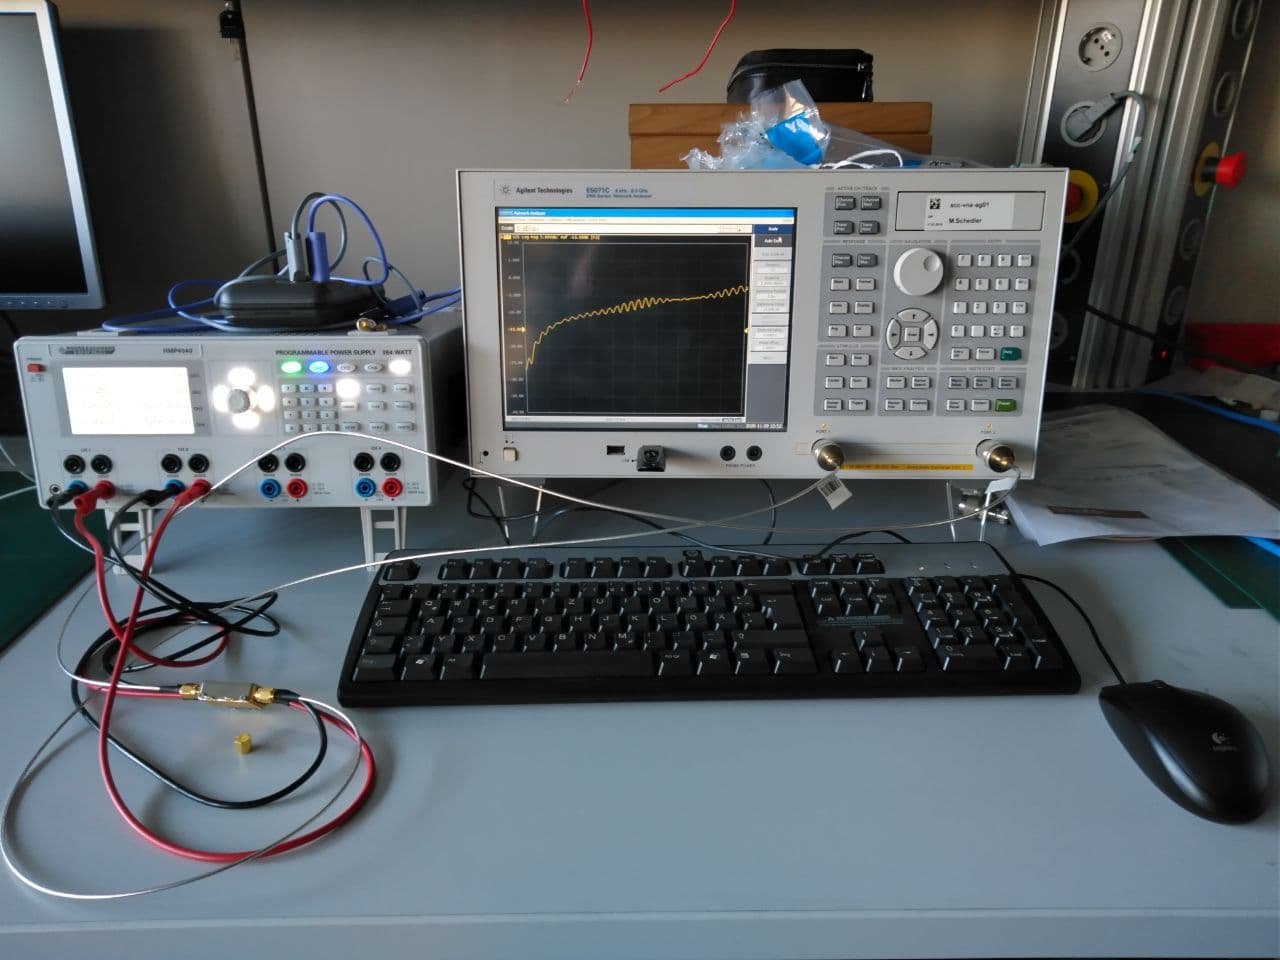
\includegraphics[width=\textwidth]{img/setup.jpg}
	\caption{The setup with power supply (left) and network analyzer (right)}
	\label{fig:setup}
\end{figure}


